\section{Hall Registrar Module: Resident Data Verification}
To ensure accurate record-keeping, the Hall Registrar utilizes a specialized queue to manage applicants who have applied for residential facilities.

\subsection{Hall Applicant Queue}
The interface displays a list of students who have cleared the academic and administrative stages and are now waiting for residential allocation.

\begin{figure}[H]
    \centering
    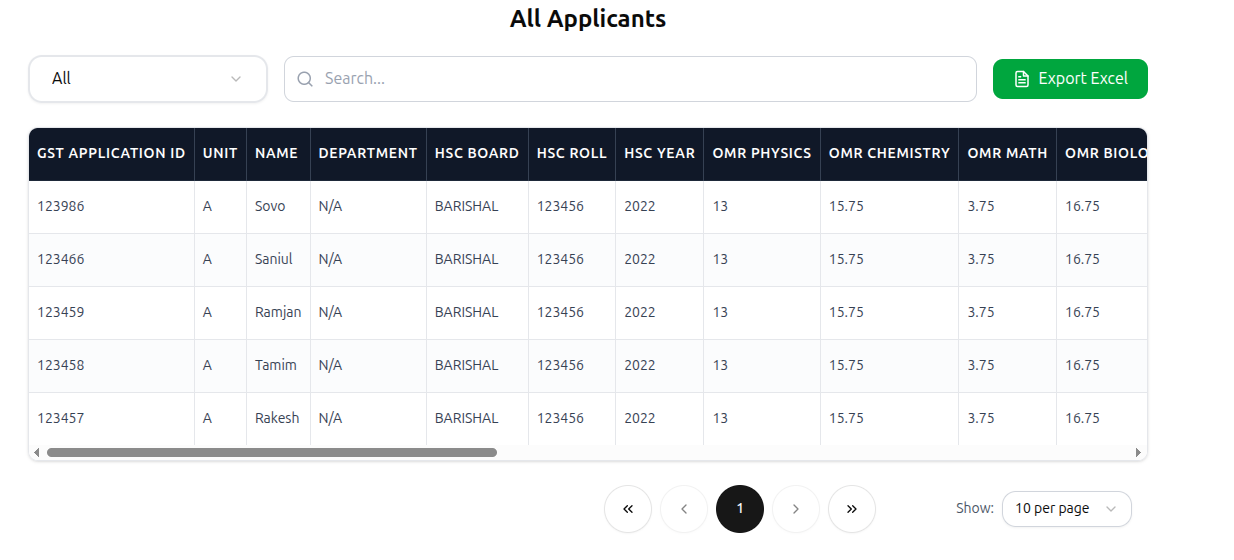
\includegraphics[width=0.9\textwidth]{chapters/chapter4/images/applicantList.png}
    \caption{Hall Resident Applicant Queue}
    \label{fig:hall_applicant_queue}
\end{figure}

\subsection{Detailed Resident Attributes}
The Hall Registrar can view specific student data, such as permanent address and gender, which are crucial factors in hall assignment.

\begin{figure}[H]
    \centering
    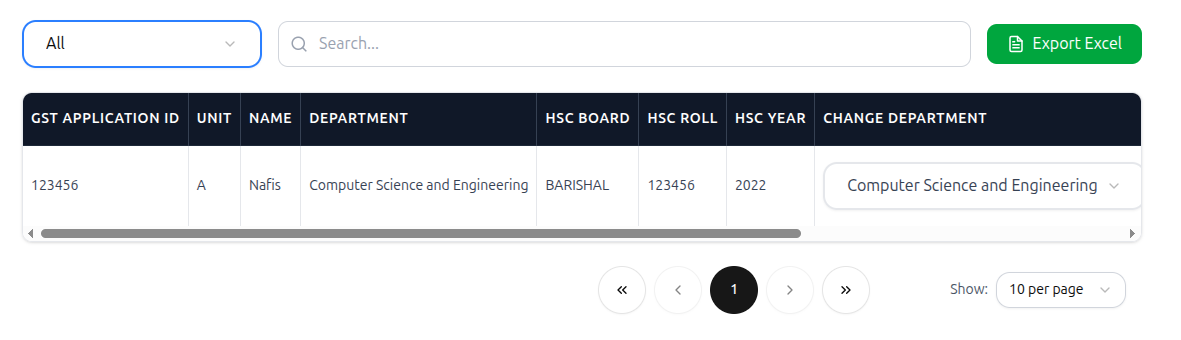
\includegraphics[width=0.9\textwidth]{chapters/chapter4/images/listTable.png}
    \caption{Detailed Resident Information Matrix}
    \label{fig:hall_resident_table}
\end{figure}